\chapter{Explainable Classifiers}\label{sec-explainable-classifier}

As discussed previously, for classification, explainability refers to the ability to explain the reasons of a classifier. To achieve explainability, existing work mainly falls into two categories. The first type of work develops more interpretable models that are easy to understand for humans. The second type of work generates explanations for a classifier without modifying the model, either by explaining the classifier locally on specific instances, or by explaining the behavior of the classifier globally.

\section{Classification}

To clarify the scope of this survey, we first briefly introduce the problem of classification, as an instance of supervised learning, and a few popular classifications models (classifiers). 

%% Briefly Introduce classification

\subsection{Definition}

Given an input space $\mathcal{X}$ and an output space $\mathcal{Y}=\{1, 2, ..., K\}$ with $K$ classes, \textbf{classification} is the problem of identifying any \textbf{observation} $\mathbf{x}\in\mathcal{X}$ to a class $y\in\mathcal{Y}$. For multi-label classification, where class labels are not exclusive, we can view it as multiple related binary classification. For simplicity, we only consider the basic formulation in this survey. 

A \textbf{classifier} is an algorithm $f$ that implements classification, \ie, $y = f(\mathbf{x})$. To handle ambiguity, a classifier is often used in a probabilistic setting. That is, the output of $f$ a probabilistic distribution $p(y\mid \mathbf{x}, \mathcal{D})$ over all possible classes in $\mathcal{Y}$. $\mathcal{D}$ is the training set, which is a subset of $\mathcal{X}\times\mathcal{Y}$, that have already been observed. Thus, in practice, a classifier will often take the form of $\mathbf{y} = f(\mathbf{x})$, where $\mathbf{y}=(y_i)\in\mathbb{R}^K$ is a vector denoting the probabilistic distribution. Then the final classification will be the class $i$ with largest probability $\arg\max_{i}{y_i}$.

Classification is now widely applied in solving many real world applications. A few examples are: face recognition [], handwritten recognition [], sentiment analysis [] and spam filtering.

% The \textbf{learning} or training of a classifier is the process of determining the best $f\in\mathbf{F}$ based on a given training set $\mathbf{D}$ that minimizes our cost of error, or, \textbf{loss function}. 

\subsection{Classifiers}

Here we briefly present a few popular models for classifications, including $k$-nearest neighbors, support vector machines, decision trees and neural networks.

\textbf{$K$-nearest neighbor}.

\textbf{Support vector machine}.

\textbf{Decision trees}.

\textbf{Neural networks}. CNN, RNN.

Before we go into details the discussion on improving explainability of classifiers, we first present an overview of the categorization.

--------

A table goes Here

--------

\section{Interpretable Classifiers}\label{sec:interpretable-classifier}

\textbf{Interpretable classifiers} are the classifiers that are commonly recognized to be more understandable than others, and hence, do not need extra explicit explanations. Summarizing existing work, we find two major strategies for creating interpretable classifiers: developing interpretable models with easy-to-understand structures, and learning simpler or sparser models.

\subsection{Interpretable Models}

To create more interpretable classifiers, a natural way is to use simple computation structures (\eg, if-then rules) in classifier. Most models that falls into this category are rule-based. 

A widely adopted type of models are the decision trees \cite{breiman1984classificationtree}. A decision tree classifier uses internal nodes and branches to represent its classification reasoning as conjunctions of rules. A human can trace back a specific classification from a leaf to the root to understand the prediction of the classifier. However, the difficulty of constructing a high-accuracy and interpretable decision tree has long been criticized. 

Focused on balancing among performance, explainability and computation, a few recent studies introduce the Bayesian framework in rule-based classifiers. Letham \etal \cite{letham2015stroke} develop the Bayesian Rule List which employs a prior structure that encourages sparsity in the generated decision lists with a good accuracy. Wang and Rudin \cite{wang2015falling} design the Falling Rule Lists that use an ordered if-then rule list so that the most at-risk occasion will be handled first. Wang \etal \cite{wang2017rulesets} construct rule sets based on AND and OR operations and highlight its low computation cost and on-par accuracy compared with SVM and random forest.

\begin{figure}[tb]
  \centering
  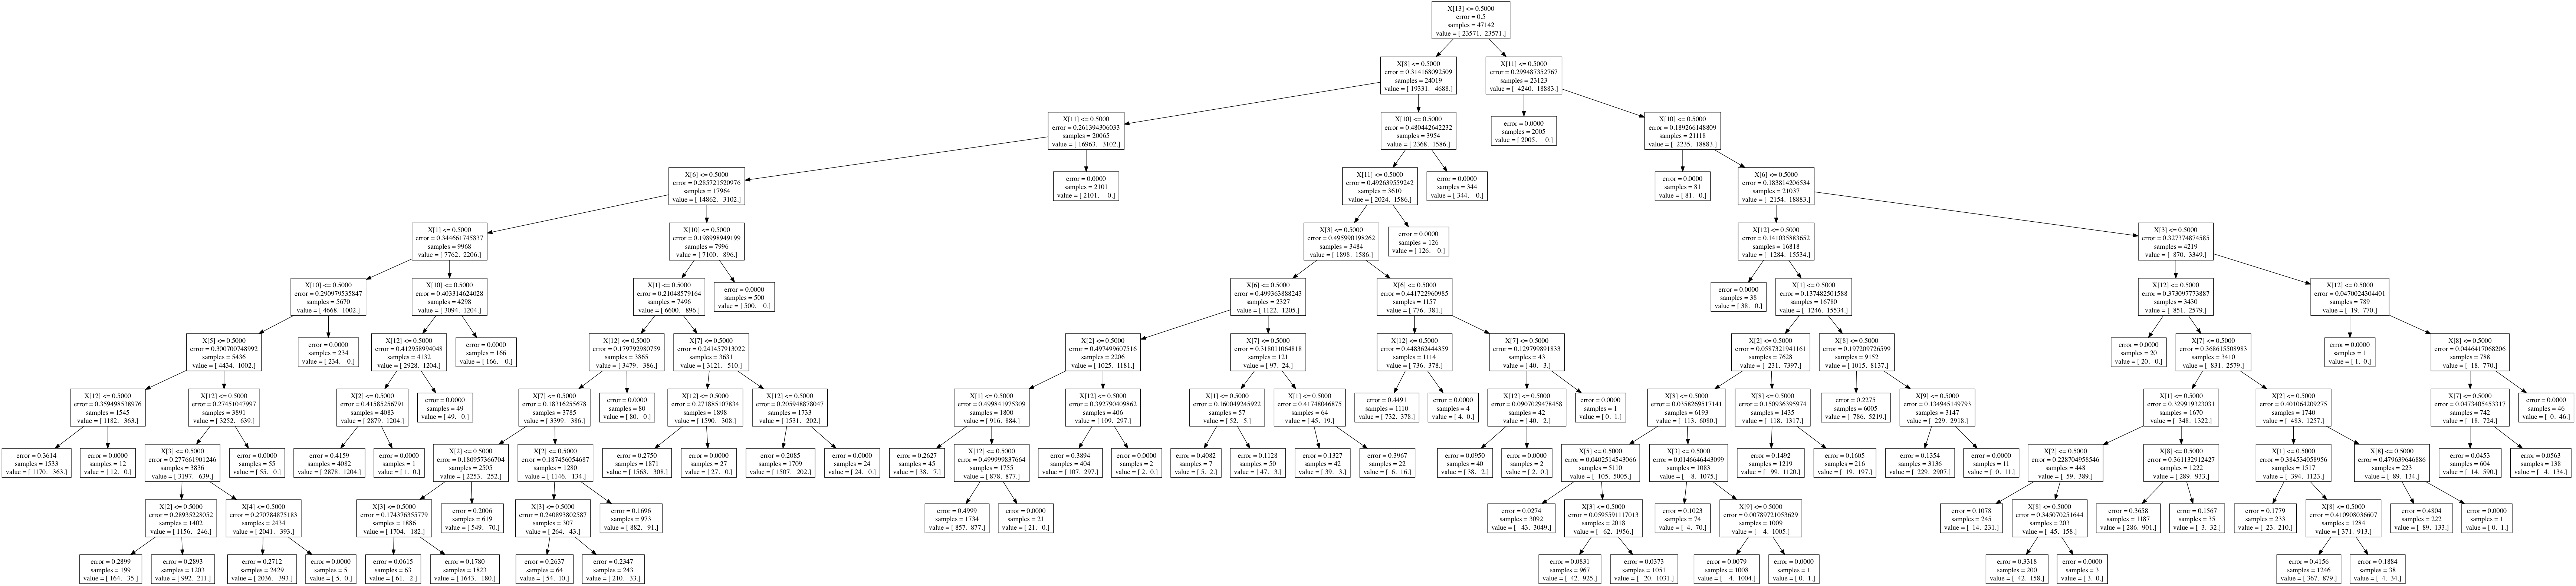
\includegraphics[width=1.0\textwidth]{figure/huge-tree}
  \caption{A decision tree with over one hundred nodes, which is hard to explain its reasoning.}
  \label{fig:huge-tree}
\end{figure}
% \footnotetext{{https://umbrella.cisco.com/blog/2013/06/13/server-side-software-and-malware-analysis/} }

The most series problem of these interpretable models with easy-to-understand structures is the scalability. The performance of the rule-based models increases as the number of rules increases or the non-linearity increases. Although the rule-based models are easy to learn and understand at the first glance, it is intractable to understand the classifier as a whole when the number of nodes of rules grows up to a few hundreds. An example is shown in \autoref{fig:huge-tree}.

Except for rule-based models, there are a few other models with more complicated models are recognized to be interpretable.
One family of interpretable models worth noticing are the generalized linear models \cite{debock2010gam}, which are pervasive in statistics and finance. Although these models can have highly nonlinear computations, the additive relation between nonlinear functions of features are believed to be easy-to-understand. However, the generalized linear classifiers can also be hard to understand when their non-linearity increased to a certain extent. The other non-probabilistic family of classifiers are the $k$-nearest neighbors (kNN) classifiers, whose prediction can be easily understood by presenting the observation's $k$-nearest neighbors. Numerous work has been done to boost the performance the kNN classifiers, including weighted kNN with different kernels \cite{dudani1976weightedknn} and fuzzy kNN \cite{keller1985fuzzyknn}. The explainability of kNN classifiers may easily fail when there lacks near neighbors for certain observations.

% \subsection{Learning Interpretable Representations}

% Instead of restricting the classifier to the combination of simple computations, some other work dedicates to learn more interpretable representations from the data. For example, Maier \etal [] learning causal knowledge from relational representations

% Features used by the model are easily interpretable.

% e.g. KNN


% Translation \cite{bahdanau2014translation}.
% Image Captioning \cite{xu15icml}.

\subsection{Learning Sparser Models}

As discussed above, the explainability often decreases as the complexity (\ie, number of parameters or nodes) of the model increases. Thus, we can improve the explainability by learning a sparser model with the same architecture. These methods can also be regarded as model compressions, which reduce computation costs. In this category, researchers develop methods that can learn a sparser model with the similar performance, usually in a per-model manner. 

% Note that learning sparse neural networks are not part of this category, since they focus on reducing the computation cost rather than explainability.

For decision trees, Quinlan summarizes four techniques for model simplification\cite{quinlan1987simplifying}, \ie, cost-complexity pruning, reduced error pruning, pessimistic pruning and simplification to rule sets. Liu \etal \cite{liu2015sparsecnn} use a sparse decomposition method to zero out redundant parameters in a CNN, which achieve about 10-times speedup while lost accuracy for only 1\%. Other simplification or methods include sparse linear integer models \cite{ustun2016supersparse}, 

...

Although 

In most cases, the efforts of developing more interpretable classifiers are tradeoffs between performance and explainability. However, for performance-critical applications,  these methods cannot provide the required explainability.

% A common problem of these interpretable classifiers, either by using simple structures or by learning sparser models, is that their explainability depends on the data itself. If the inputs $\mathbf{x}$ are intrinsically difficult to explain,

\section{Explanation of Classifiers}
(4 pages)

\subsection{Definitions of Explanation}

A review of how previous work define explanations in machine learning.

General: ML:\cite{doshi-velez2017interpretableml}. Cognitive:\cite{lombrozo2006explanation}

Data-type specific definitions: image-based, text-based, categorical data.

Some other work focuses on explaining the model itself (the mechanism, compositions of the model) to facilitate the understanding and diagnosing of the model.

To summarize, no agreed definition of explanation of classifier exists. Here we give a general definition...Next we give problem specific definitions.

Learned from surveying the literature, we separate the problem of explaining classifiers into two sub-tasks: explaining the predictions of classifiers (instance-level); explaining the classifier itself (model-level).

% For each sub-tasks, the existing methods can be divided into two types: model-aware explanations and model-unaware explanations.


\subsection{Local Explanation}
Brief intro.

\textbf{Model-aware methods}

image data: \cite{simonyan14saliency,zeiler2014eccv,bach15plos,zintgraf17visualize}

text data: \cite{karpathy16rnn,li2016naccl-hlt,martens2014explaindocument,arras2017rnn-sentiment}

\textbf{Model-unaware methods}

  - Learn to explain (Image captioning) \cite{hendricks16generate}

  - Model induction (Locally approximate) \cite{ribeiro2016kdd}

  - Trace back to training data (influence function) \cite{pang2017influencefunctions}
 
\subsection{Global Explanation}
Brief intro.

\textbf{Explain inner components of the model} (model-aware) 

RNN: \cite{ming2017vast}

CNN: \cite{bau2017netdissect} study interpretable units

NN: \cite{feraud2002nn}

\textbf{Explain the model as a whole} (model-unaware) 

\cite{ribeiro2016kdd} Image and text, sampling instanc-level explanations

\cite{martens2014explaindocument} Text


\section{Evaluation}

Address the problem of evaluation, and how other work evaluates.

\newpage